

\section{Thermal Effects on Repository Performance}
\subsection{Decay Heat}

The radioactive decay of isotopes in spent nuclear fuel produces heat. The 
activity of a radioactive sample is equal to the sum of the activities of each 
of its constituent isotopes. In Bequerels, or disintegrations per second, 
radioactivity is expressed in terms of the decay constant, 

\begin{align}
A_{sample} &= \sum_i^{n}A_i\nonumber\\
           &= \sum_i^{n}\lambda_i N_i
\intertext{where}
A_{sample} &= \mbox{ disintegrations per second in the sample }[Bq]\nonumber\\
A_{i} &= \mbox{ disintegrations per second due to isotope i }[Bq]\nonumber\\
n    &= \mbox{ the number of isotopes species in the sample }[-]\nonumber\\
\lambda_i    &= \mbox{ the decay constant of isotope i }[Bq]\nonumber\\
N_i    &= \mbox{ the number of atoms of isotope i in the sample }[-].\nonumber
\end{align}

The specific activity of a sample, defined as the activity per unit mass, is 
then 

\begin{align}
  SA &= \sum_i^n SA_i\nonumber\\
     &= \sum_i^n\frac{\lambda_i N_{Av}}{M_i} 
  \label{sa}
  \intertext{where}
  N_{Av} &= \mbox{ Avogadro's number } 6.022\times10^{-23}[mol^{-1}]\nonumber\\
  M_i &= \mbox{ Atomic weight of isotope i } [g\cdot mol^{-1}].\nonumber
\end{align}

The specific power, in $MeV\cdot s^{-1} \cdot g^{-1}$ generated by that sample 
at that second employs an isotope specific energy per disintegration factor,

\begin{align}
  p &= \sum_i^n\frac{E_i \lambda_i N_{Av}}{M_i}[MeV\cdot s^{-1} \cdot g^{-1}]
  \label{specpower}
  \intertext{where}
  E_i &= \mbox{ Average energy release per disintegration of isotope i }[MeV].\nonumber
\end{align}

Energy in $MeV$ can be converted to Watts by the conversion factor,

\begin{align}
  1 [MeV\cdot s^{-1}] = 1.6\times10^{-13}[W],
  \label{MeV2Watt}
\end{align}
such that the total heat of a sample can be expressed as 
\begin{align}
  Q &= \sum_i^n 1.6\times10^{-13}\frac{I_i E_i\lambda_i N_{Av}}{M_i}[W]
  \label{totHeat}
  \intertext{where}
  I_i &= \mbox{ the inventory of isotope i in the sample } [g].\nonumber
\end{align}

This gives only the instantaneous decay heat production of a sample. To arrive 
at long term decay heat curves, decay heat contributions from the chain of 
daughter products must be calculated as well. Typically, the latter calculation is 
done by detailed depletion codes. 




\subsection{Capacity Determination for Arbitrary Waste Form}

Modeling heat will require a transient model capable of arriving at a heat based 
capacity quickly for an arbitrary waste stream. 

Superposition of known, mass normalized, decay heat evolution curves will 
result in a heat source term curve for the waste form for future times,

\begin{align}
Q(t) &= \sum_{i=0}^{n}I_iq_i(t)
\label{heatsource}
\intertext{where}
Q(t) &= \mbox{ Total waste form heat at time t }[W]\nonumber\\
i &= \mbox{ Index of the isotope species }[-]\nonumber\\
n &= \mbox{ Number of isotopes in the waste form }[-]\nonumber\\
I_i &= \mbox{ Inventory of isotope i in the waste form }[g]\nonumber\\
q_i(t) &= \mbox{ Heat due to one gram of i after time t }[W\cdot g^{-1}].\nonumber
\end{align}

Determination of $q_i(t)$ must come from tabulated and mass normalized results 
of depletion calculations, or otherwise available decay heat curves for heat 
generating nuclides and their daughters.

With this algebraic calculation of $Q(t)$, the heat evolution of the waste form, 
there are a number of approximations that may assist in estimating repository 
capacity for that waste stream while holding the package spacing constant. 

\subsubsection{Areal Power Density Approximation}

A uniform areal power density can be used to determine appropriate repository 
loading for arbitrary waste streams. 

\begin{figure}[htbp!]
\begin{center}
      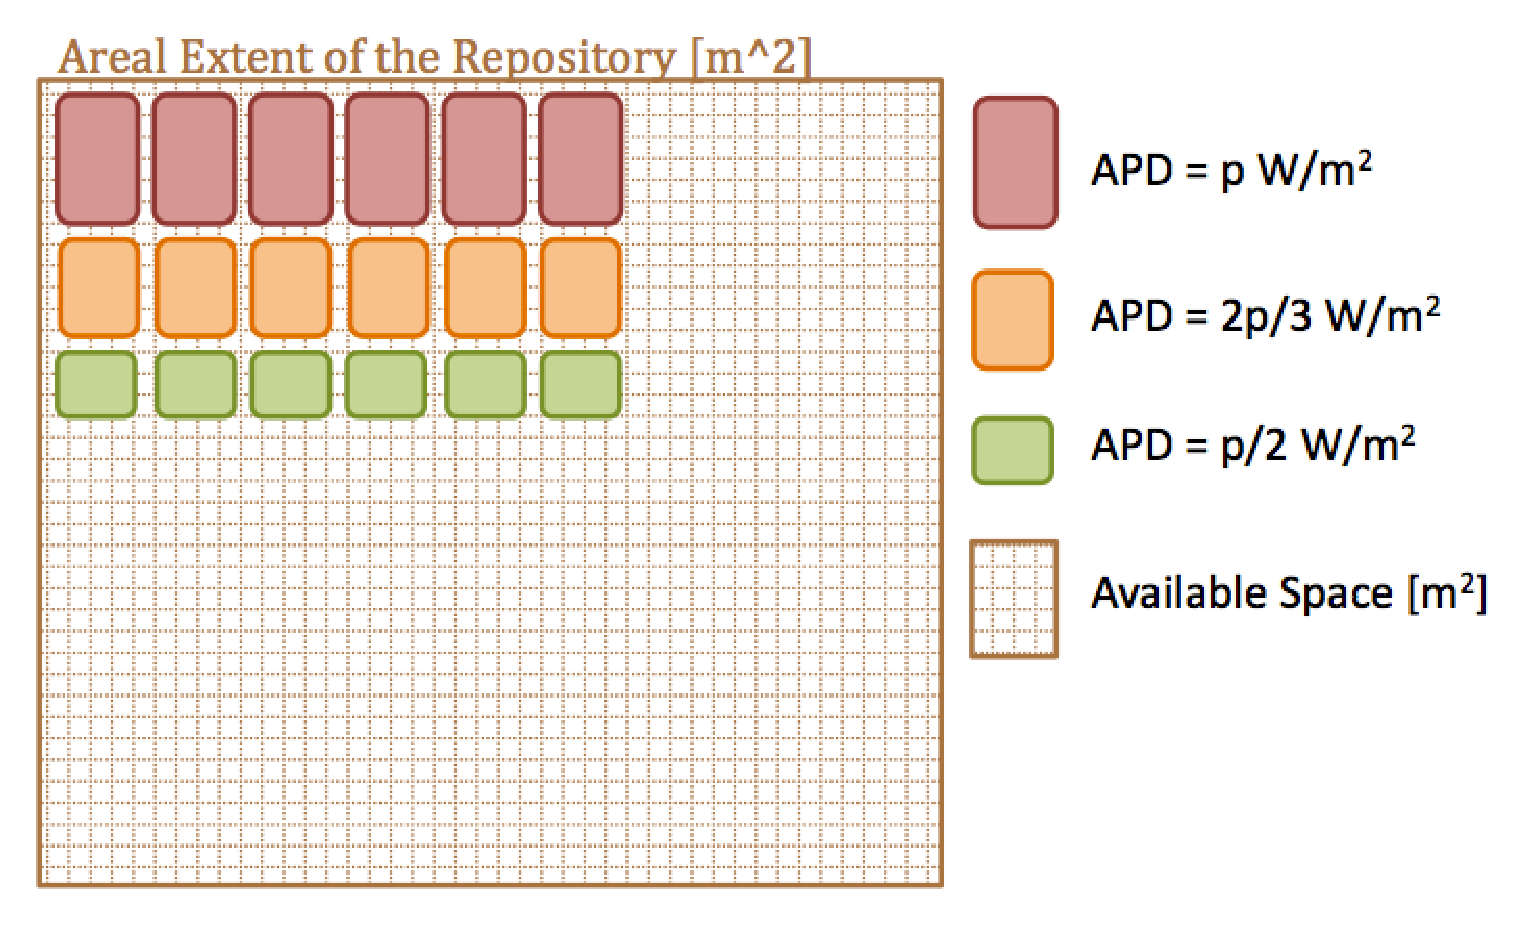
\includegraphics[width=0.7\textwidth]{APD.eps}
      \caption{The areal power density loading scheme pictured above is not 
      constrained by uniform spacing and takes advantage of denser spacing 
      made possible by cooler packages (green).  }
      \label{fig:apd}
      \end{center}
\end{figure}

In the areal power density loading schem, loading is subject to the constraints,
    \begin{align}
      P_{tot} &\le P_{max} \\
      APD_i &\le APD_{max}
      \intertext{where}
      P_{max} &= A\cdot APD_{max}\\ 
      P_{tot} &= \sum_{i=0}^{N}n_i P_i\\ 
      P_i &= \mbox{power of package i}\nonumber\\
      n_i &= \mbox{ith package}\nonumber\\
      N &= \mbox{number of packages}\nonumber\\
      APD_{max} &= \mbox{max areal power density}\nonumber
    \end{align}

\subsubsection{Peak Heat Approximation}

One conservative estimation could assume that $Q(t)$ is a constant heat flux, 
$Q_{max}$ equal to the peak of calculated waste form heat evolution, 
$max(Q(t))$. Assuming $Q(t) = Q_{max} \forall t$, it would be possible to 
directly refer to previously calculated repository evolution results 
based on constant heat and spacing. 

\begin{figure}[htb!]
  \begin{center}
    \def\svgwidth{.7\textwidth}
    \input{acceptance.eps_tex}
  \end{center}
  \caption{Above the empirically determined acceptance threshold for a certain 
  $K_{th}, \alpha_{th}$ combination, the arbitrary  waste stream is likely to be 
  acceptable. Below it, the waste stream is likely to be unacceptable. }
  \label{fig:acceptance}
\end{figure}

\subsubsection{Heat Integral Approximation}

Another approximation could develop the heat and spacing thresholds based on the 
integral of heat over time. Then, the time evolution of $Q(t)$ could be captured  
in the comparison. 

\begin{figure}[htb!]
  \begin{center}
    \def\svgwidth{.7\textwidth}
    \input{acceptanceInt.eps_tex}
  \end{center}
  \caption{Above the empirically determined acceptance threshold for a certain 
  $K_{th}, \alpha_{th}$ combination, the arbitrary  waste stream is likely to be 
  acceptable. Below it, the waste stream is likely to be unacceptable. }
  \label{fig:acceptanceInt}
\end{figure}

One method in the literature not dissimilar to this is the Specific Temperature 
Integral by Jun Li\cite{li_specific_2008}. 

A specific temperature integral may model the thermal source as linear along the
emplacement paths, analagously to the areal power density method.
However, a temperate integral takes account of heat transfer behavior in the
rock, includes the effects of myriad SNF compositions, and gives the thermal
integration over time for any specific location within the rock.  Man-Sung Yim
calls this the Specific Temperature Increase method\cite{li_specific_2008}.

In the same way that $Q(t)$, the heat flux from the waste streams, can be
expressed as the superposition of the linear heat flux contributions of all the
radionuclides in the waste, he temperature change
expressed as a superposition of the temperature change contributions due to  
each radionuclide. Each radionuclide contributes in proportion to its
decay heat generation and its weight fraction of the SNF. With information
about isotopic composition of the SNF, the specific temperature increase can
determine the maximum thermal capacity of the repository in terms of tonnes/m.
The length based accounting in $\frac{t}{m}$ is converted to
$\frac{t}{Repository}$ by multiplication with the total emplacement tunnel
length of the repository. 

\subsubsection{Effective Mean Decay Power}

Introduced by Radel, Wilson et. al., the Specific Temperature Change method uses 
a linear approximation to arrive at the thermal loading density limit.  

The mean decay constant of the radionuclide constituents in the waste form was 
compared to the thermal time constant in the rock. 

When the thermal time constant of the rock is much shorter than the waste form 
decay package, the change in package wall temperature can be described by 

\begin{align}
q(t_0)\rho_{limit}C'&=\Delta T_1
\label{fig:Tracyfig}
\intertext{where}
\rho_{limit} &= \frac{C_1}{Q_1}\nonumber\\
C' &= \mbox{ Thermal constant }[-]\nonumber\\
\Delta T &= \mbox{ Constant difference between }T_{lim}\mbox{ and }T_{amb}[^{\circ}C]\nonumber\\
T_{lim} &= \mbox{ Temperature limit }[^{\circ}C]\nonumber\\
T_{amb} &= \mbox{ Ambient rock temperature }[^{\circ}C]\nonumber
\end{align}

\subsubsection{Thermal Half-Life Approximation}

There is some notion of a thermal halflife in the literature. 



\subsection{Waste Stream Loading Density in Waste Forms}

Either the user inputs the waste form loading density or the repository must 
determine how best to load the waste forms with waste .

\subsection{Waste Package Loading Strategy in Repository}

Either the user inputs the tunnel spacing and waste package spacing, or the 
repository must determine how best to space the tunnels and packages.

\subsection{Solving for the Heat Evolution}

This model should be capable of calculating the temperature field through the 
repository over time for a certain waste package layout. 

